\chapter{Warstwa API}
\label{chap:api}

\section{Struktura bazy danych}

Na rysunku \ref{fig:db-diagram} przedstawiono schemat relacyjnej bazy danych aplikacji NetHelt. Diagram obrazuje strukturę tabel oraz relacje pomiędzy encjami systemu. Schemat bazy jest tworzony i aktualizowany za pomocą migracji narzędzia Flyway.

Centralnym elementem modelu jest tabela \texttt{users}, przechowująca dane logowania użytkowników wraz z przypisaną rolą (\texttt{USER} lub \texttt{ADMIN}). Dane profilu, takie jak nazwa użytkownika, imię czy nazwisko, zapisywane są w osobnej tabeli \texttt{profiles}. Konta powiązane z zewnętrznymi dostawcami tożsamości (Google, GitHub) przechowywane są w tabeli \texttt{user\_identities}, a tokeny odświeżania sesji oraz tokeny resetowania hasła w tabelach \texttt{refresh\_tokens} i \texttt{password\_reset\_tokens}.

Każdy użytkownik może posiadać wiele sieci, zapisanych w tabeli \texttt{networks}. Do każdej sieci przypisany jest jeden agent (\texttt{network\_agents}), czyli klient desktopowy zainstalowany w tej sieci. Tabela przechowuje skrót tokenu dostępowego agenta, czas ostatniego sygnału aktywności (\emph{heartbeat}) oraz maksymalny czas niedostępności, po którego przekroczeniu użytkownik otrzymuje powiadomienie. Urządzenia sieciowe zapisywane są w tabeli \texttt{devices} i również należą do konkretnej sieci. Adres IP urządzenia przechowywany jest dodatkowo w postaci liczbowej, co umożliwia szybkie filtrowanie urządzeń według zakresu adresów.

Z każdym urządzeniem powiązane są zadania monitorujące (\texttt{monitoring\_tasks}), określające typ wykonywanej operacji (\texttt{PING}, \texttt{TELNET} lub \texttt{HTTP\_HEALTHCHECK}), odstęp czasu pomiędzy kolejnymi wykonaniami oraz to, czy wyniki zadania podlegają analizie przez moduł AI. Parametry zależne od typu zadania, np. port czy oczekiwany kod odpowiedzi HTTP, zapisywane są w osobnych tabelach konfiguracji (\texttt{ping\_task\_configurations}, \texttt{telnet\_task\_configurations}, \texttt{http\_healthcheck\_task\_configurations}), powiązanych ze wspólną tabelą \texttt{monitoring\_task\_configurations}.

Wyniki wykonanych zadań zapisywane są w tabeli \texttt{monitoring\_results}, gdzie gromadzone są informacje o powodzeniu operacji, czasie odpowiedzi oraz momencie wykonania. Para kolumn \texttt{task\_id} i \texttt{executed\_at} jest unikalna, dzięki czemu wyniki ponownie wysłane przez agenta po odzyskaniu połączenia nie są zapisywane podwójnie. Dane specyficzne dla typu zadania, takie jak stan portu lub otrzymany kod odpowiedzi HTTP, przechowywane są analogicznie w tabelach rozszerzeń wyników (\texttt{monitoring\_result\_extensions} i tabelach pochodnych). Na podstawie zgromadzonych wyników tworzone są jednominutowe okna czasowe, przekazywane do analizy do modułu AI. Wynik analizy każdego okna, wraz z informacją o wykryciu anomalii oraz wersją modelu, zapisywany jest w tabeli \texttt{ai\_analysis\_results}.

Wyniki wykrywania urządzeń w sieci lokalnej przechowywane są w tabelach \texttt{discovery\_scans} oraz \texttt{discovery\_scan\_results}. Pierwsza z nich opisuje skanowanie zlecone przez użytkownika, w tym zakres adresów i jego status, a druga adresy IP oraz nazwy urządzeń, które odpowiedziały w trakcie skanowania.

Powiadomienia przechowywane są w tabeli \texttt{notifications}, a informacje o ich dostarczeniu poszczególnymi kanałami (e-mail, aplikacja webowa, Telegram) w tabeli \texttt{notification\_deliveries}. Tabela ta zapisuje również liczbę prób wysyłki oraz ostatni błąd, co umożliwia ponawianie nieudanych wysyłek. Kanały wybrane przez użytkownika zapisywane są w tabelach \texttt{notification\_preferences} i \texttt{notification\_enabled\_channels}, natomiast powiązanie konta użytkownika z komunikatorem Telegram w tabeli \texttt{telegram\_accounts}. Reguły określające, jakie zdarzenia wywołują alert, np. kilka nieudanych prób z rzędu lub przekroczenie progu czasu odpowiedzi, przechowywane są w tabeli \texttt{alert\_rules}. Błędy aplikacji serwerowej zapisywane są w tabeli \texttt{error\_logs}, udostępnianej administratorowi do przeglądania.

Tabele \texttt{users} oraz \texttt{networks} posiadają kolumnę \texttt{deleted\_at}, która pozwala na wykonywanie miękkich usunięć z systemu, co ułatwia utrzymanie integralności danych i umożliwia przywrócenie usuniętego konta. Unikalność adresu e-mail oraz nazwy sieci sprawdzana jest wyłącznie wśród rekordów, które nie zostały usunięte.

Kolumny takie jak \texttt{role}, \texttt{type}, \texttt{status} czy \texttt{channel} są ograniczone do predefiniowanych wartości, które w kodzie źródłowym programu występują jako typ wyliczeniowy. Pozwala to uniknąć błędnego wprowadzenia danych poprzez wyświetlenie odpowiedniego komunikatu błędu.

\begin{figure}[H]
	\centering
	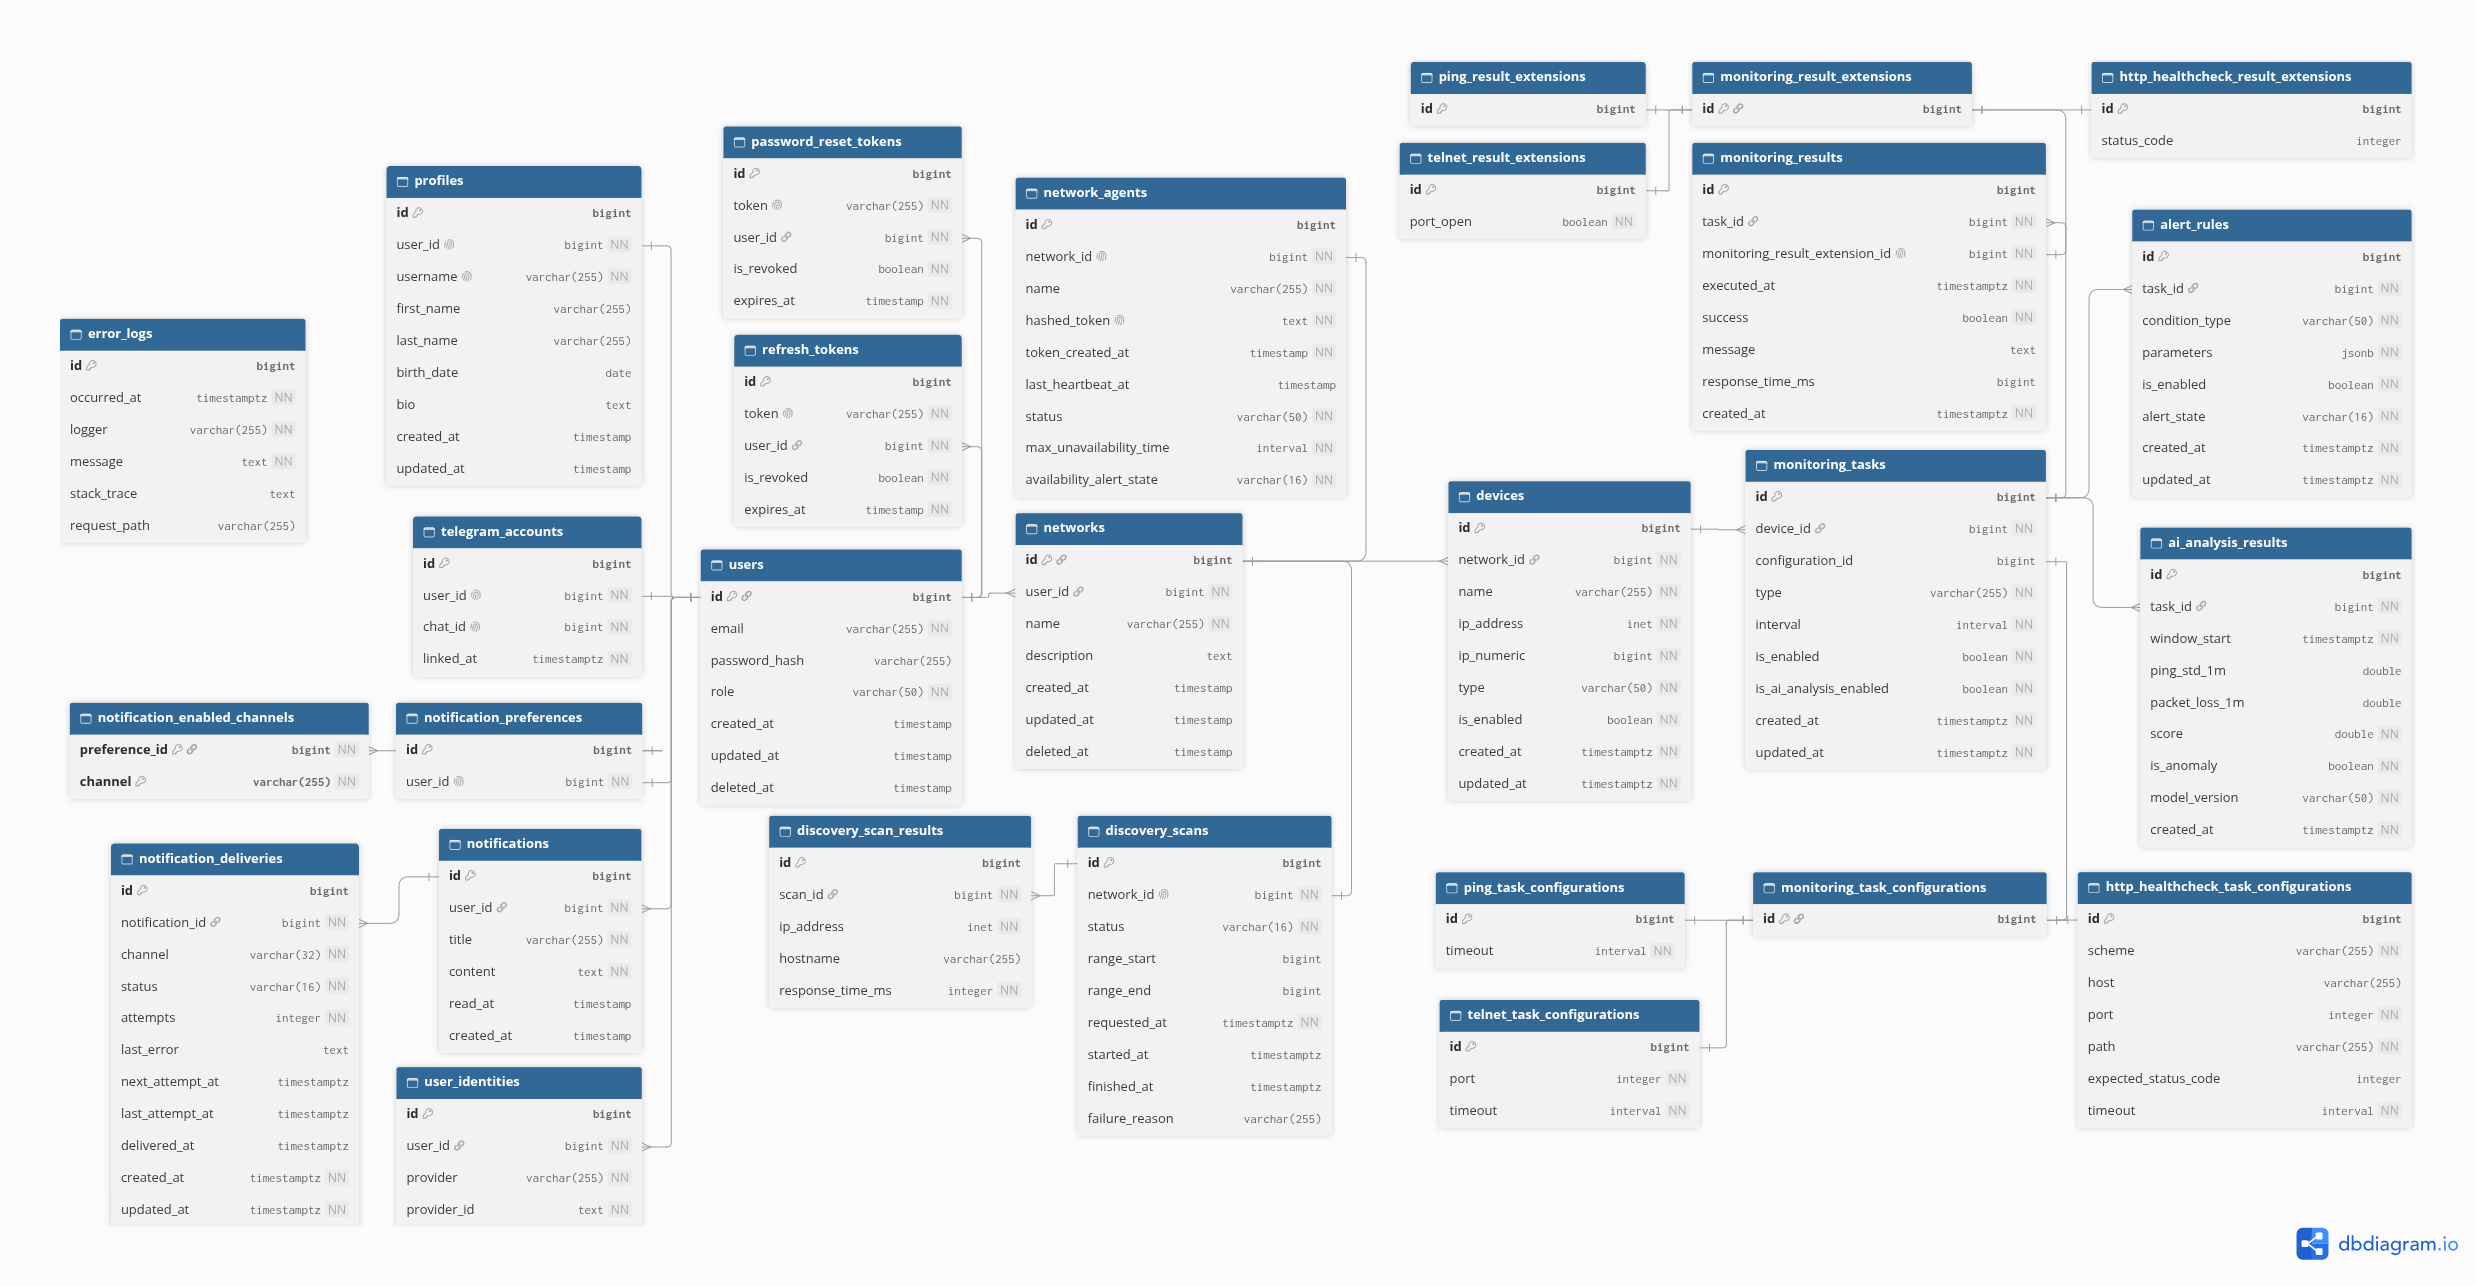
\includegraphics[width=1.0\textwidth]{./images/nethelt-db-diagram.png}
	\caption{Diagram bazy danych aplikacji NetHelt\\Źródło: Opracowanie własne w witrynie internetowej https://dbdiagram.io/}
	\label{fig:db-diagram}
\end{figure}